% $Id$

%==============================================================================
\section{Remote Component Structure}
%==============================================================================

While we have implemented a local version of CORBA Components, 
the LwCCM specification defines remote components only.
Remote components are built up from CORBA objects that implement defined
IDL interfaces.
Because of the specified mapping from IDL3 to IDL2, the generated IDL2 files 
can be processed by every existing IDL compiler. In addition to CORBA stubs
and skeletons, remote component logic as well as CORBA component containers
must be implemented too. 
To be compliant to the LwCCM specification, we have developed a way to
adapt local components into remote LwCCM components - the 
{\bf Local Component Adapter Concept} (LCAC).

LCAC allows to add remote communication
for each port transparently for business logic.
Fig.~\ref{LcacOverview} shows how a given local component implementation
can be extended to a remote LwCCM component.

\begin{figure}[htbp]
    \begin{center}
    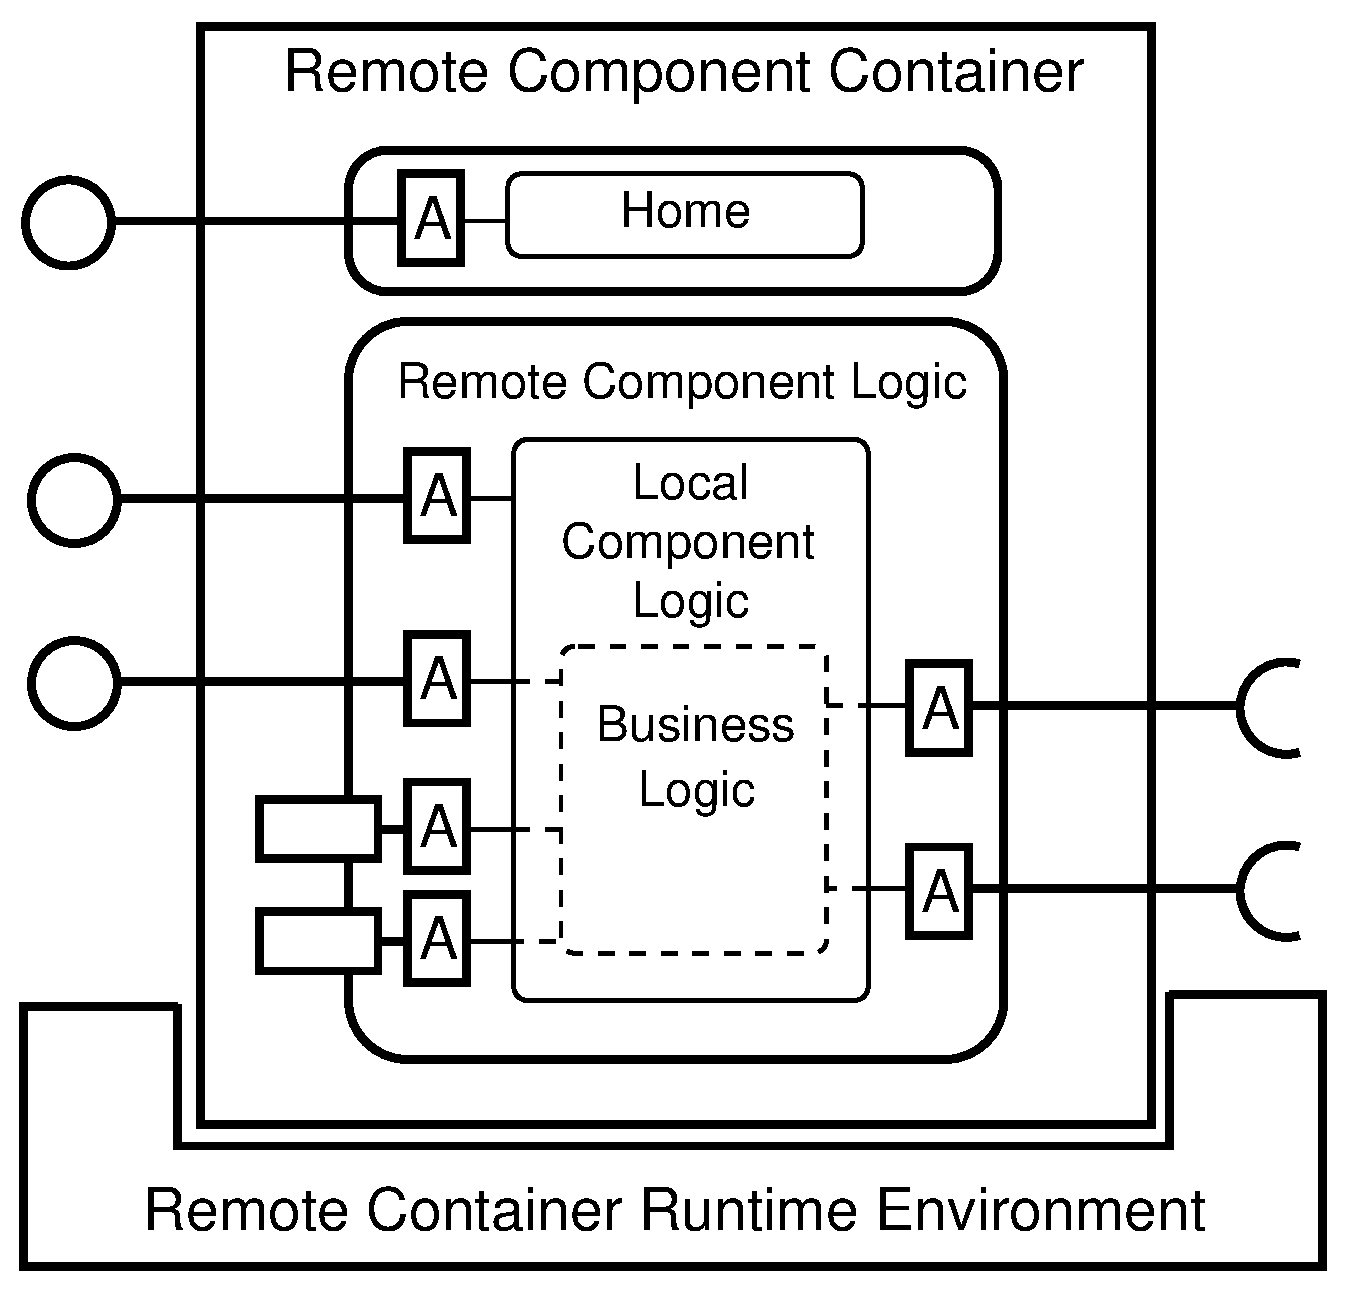
\includegraphics [width=5.5cm,angle=0] {figures/LocalAdapterConcept.eps}
    \caption{A local component can be embedded in a remote component logic
    that will be managed by a remote component container.}
    \label{LcacOverview}            
    \end{center}
\end{figure}

\noindent
The point is that we can use local components without changing them.
Thus, for a remote accessible component that provides at least one remote 
port, some additional code will be involved.

\begin{description}
\item [Remote component logic.]
A glue code layer is responsible for embedding a local component into a 
remote CORBA component. 
This remote component logic hosts a local component.
That means, its local component logic and business logic.  
Such a structure ensures that local ports can be used side by side to remote
ports.

\item [Adapter set.]
For a given IDL interface that defines a component port's syntax, a local and 
a remote implementation is generated. 
Using a set of adapter classes, these two worlds can fit together transparently.
In addition to component ports, adapters must be provided for component homes
as well as the component's equivalent interface.

\item [Remote component container.]
For each remote component type, a generic component container is used to
manage CORBA component instances.
In contrast to a local component container that can have a simple structure, a
remote container is also responsible for sophisticated {\it Quality of Service} 
(QoS) tasks.

\item [Remote container runtime environment.]
With increasing QoS functionality, the requirements to a remote container
runtime environment are growing too.
Besides an {\it Object Request Broker} (ORB), that handles CORBA requests,
libraries for multi--threading and process management implementation must 
be available.  
\end{description}

\noindent
This adapter concept is a powerful tool especially in heterogeneous 
environments. Besides the choice between local and remote connections, 
a deployment process can also decide to use different middleware technologies.


The fact that a local component is wrapped by a remote component becomes 
obvious from Fig.~\ref{StructureOfRemoteComponents}. All classes of a local
component remain unchanged, while some new ``remote'' classes have been added.

\begin{figure}[htbp]
    \begin{center}
    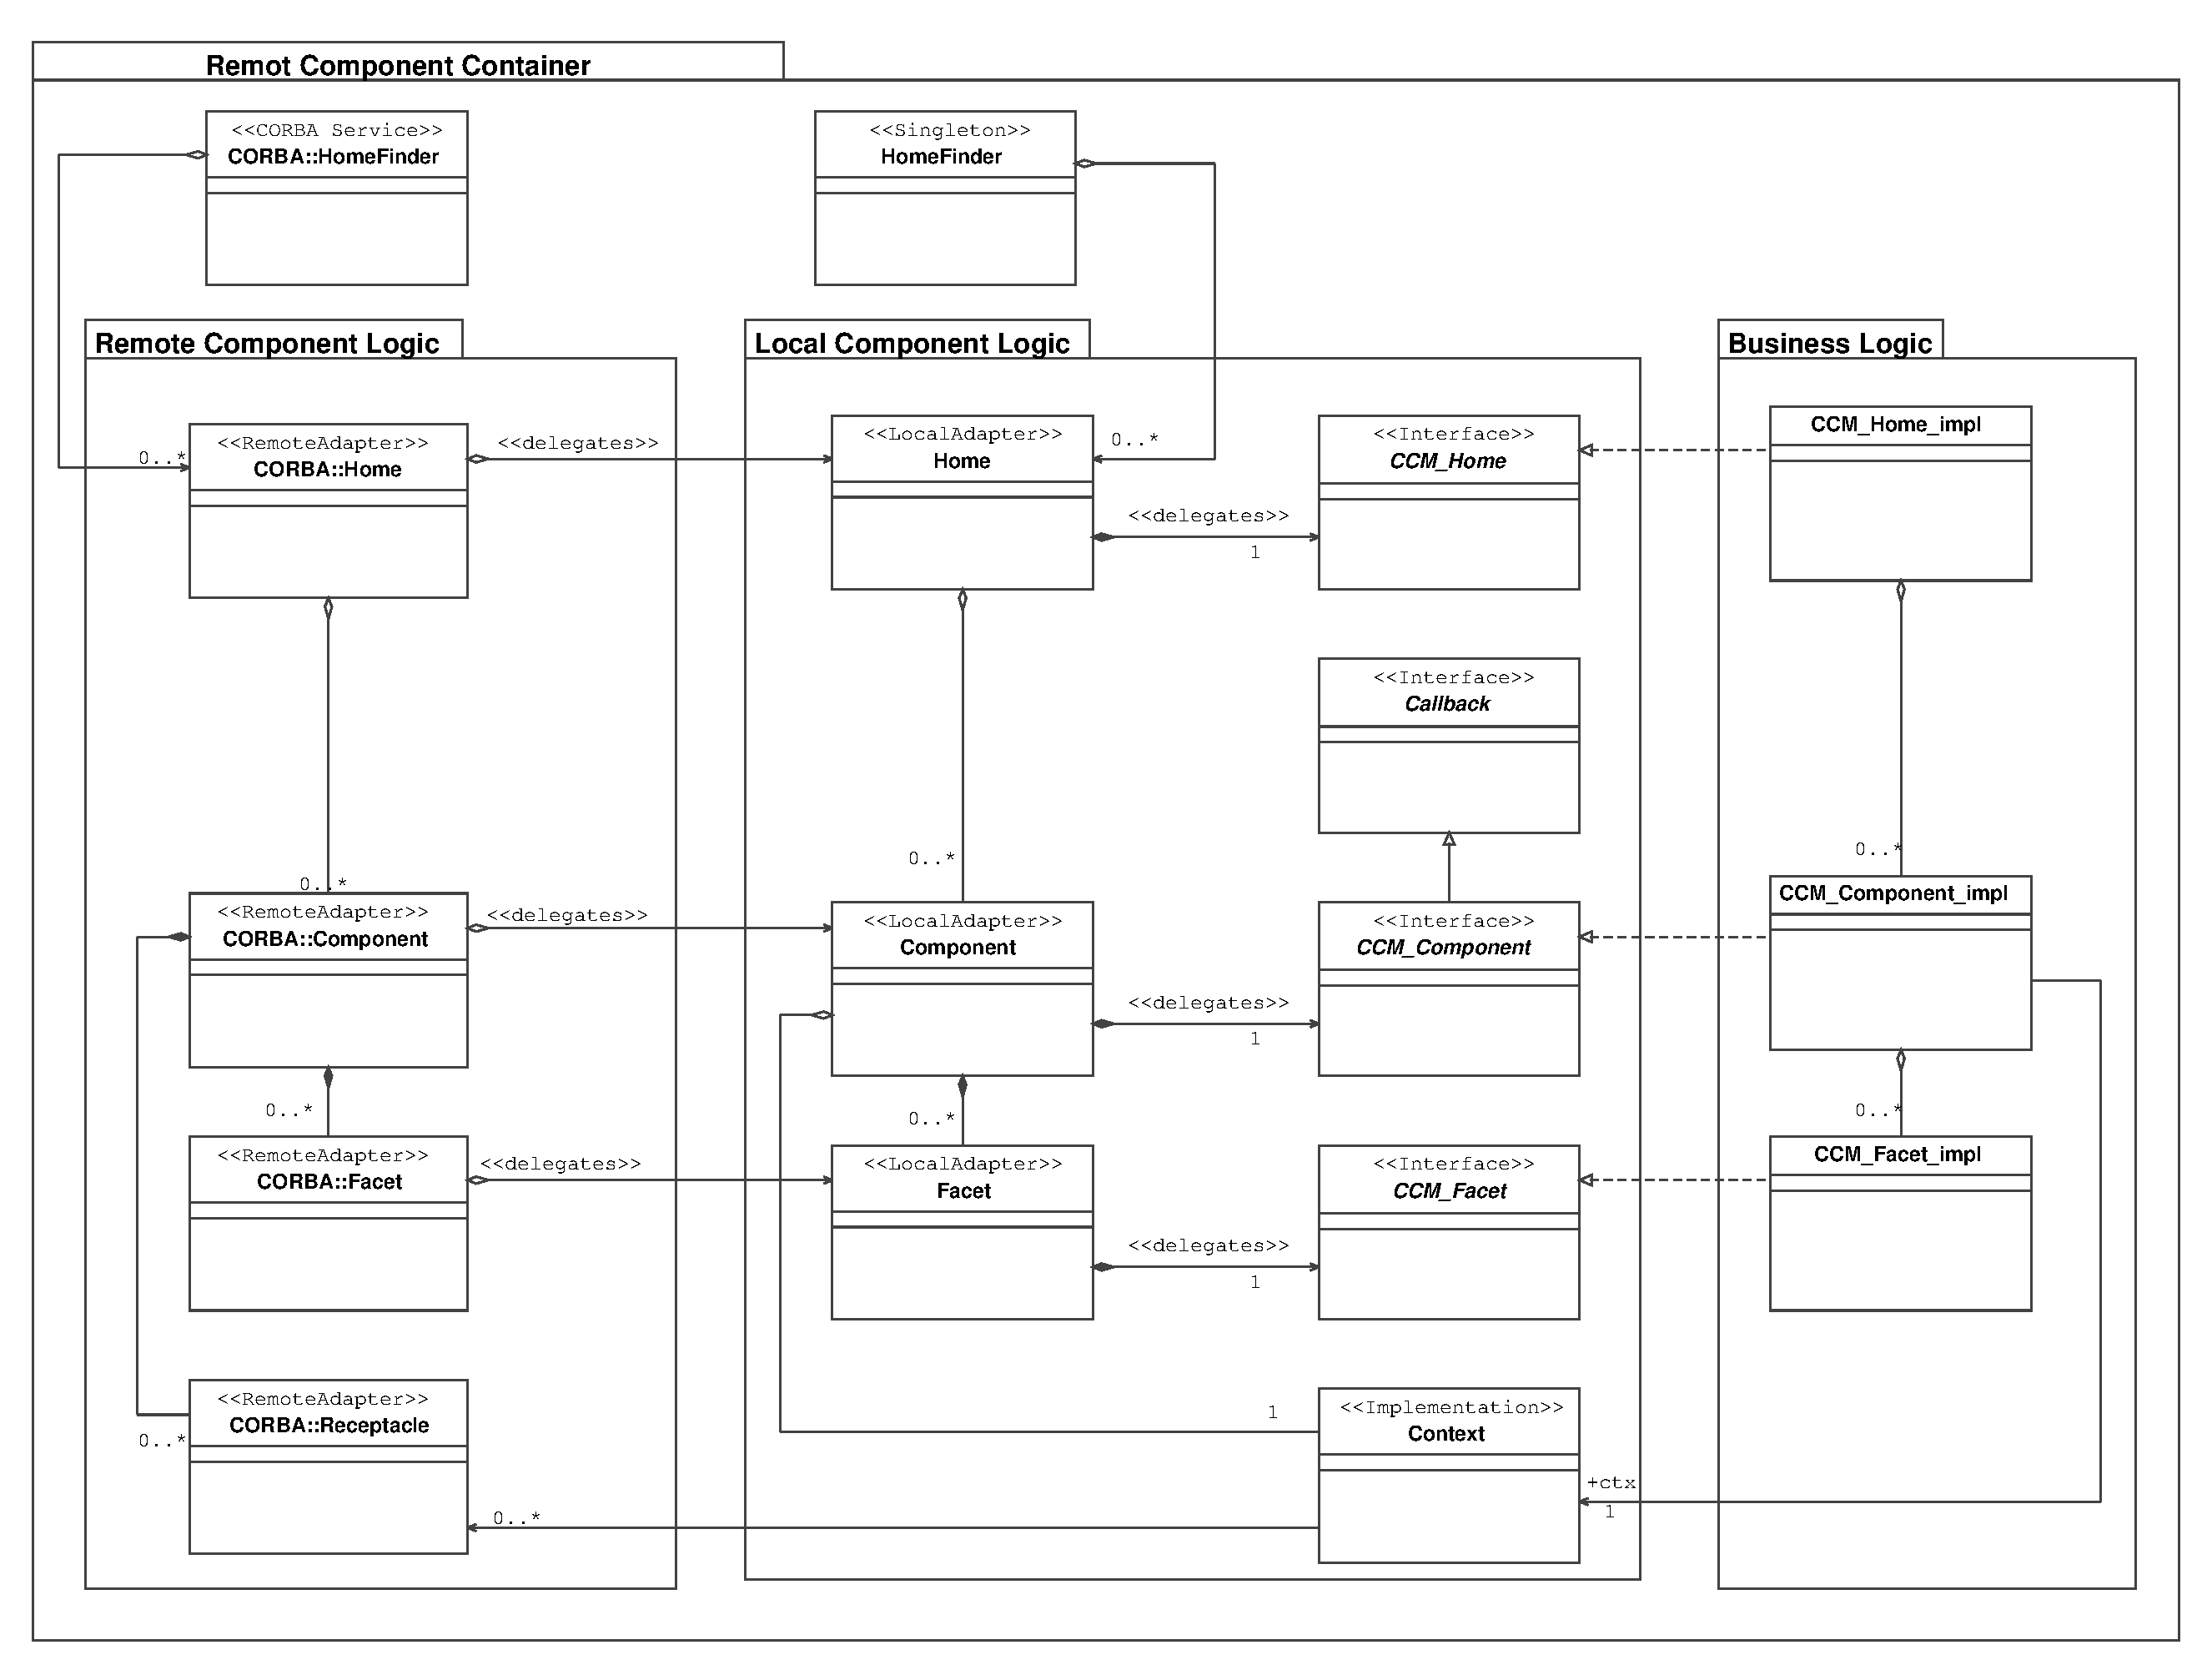
\includegraphics [width=15cm,angle=0] 
		     {uml/StructureOfRemoteComponents.eps}
    \caption{Simplified structure of a remote component implementation,
    showing the relationship between corresponding local and remote components.}
    \label{StructureOfRemoteComponents}            
    \end{center}
\end{figure}

\noindent
The remote structure is very similar to a local component's structure 
(Fig.~\ref{StructureOfLocalComponents}), thus, we can compare interactions
between a local and a remote component with interactions between business logic
and local component logic:

\begin{description}
\item [Calling component methods.]
A remote client calls methods on a remote adapter that delegates this
calls to a local component which uses a local adapter to delegate these calls
to business logic.
In each adapter, pre- and a post-invoke processing can take place 
(Fig.~\ref{RemoteComponentCall}).
\begin{figure}[htbp]
    \begin{center}
    \includegraphics [width=9cm,angle=0] 
		     {figures/RemoteComponentCall.eps}
    \caption{A remote call of a component's method is delegated twice
    allowing pre- and post-invoke processing.}
    \label{RemoteComponentCall}            
    \end{center}
\end{figure}

These two indirection layers allow non--functional extensions to 
components without changes in business logic. 
This separation of concerns is a cornerstone in component
based development.

\item [Invoking callback methods.]
Callback methods implemented by business logic can be
triggered either from local or remote component logic and their corresponding
container implementations to control a component's life cycle.

\item [Using context methods.]
Component business logic uses the {\tt Context} object to access container
functionality as well as component receptacles.
In the case of remote components, receptacles can be either local or remote
ports. Both kinds of receptacles can be accessed via local context
object methods. While local receptacles are connected directly to local facets,
remote receptacles are intercepted by a receptacle adapter.
\end{description}

\noindent
Based on LCAC, an existing LwCCM container implementation could be used to host 
local components, thus, we could combine an existing CORBA application server 
with the presented extensions in the context of local components. 

